%!Tex Root = ../main.tex
% ./Packete.tex
% ./Design.tex
% ./Deklarationen.tex
% ./Vorbereitung.tex
% ./Aufgabe2.tex
% ./Aufgabe3.tex
% ./Aufgabe4.tex
% ./Appendix.tex

\section{Aufgabe 1}

\setcounter{exercise}{1}

\begin{frame}[allowframebreaks]{Aufgabe \thesection}{Logikfunktionen}
  \begin{solution}
    \resizebox{\textwidth}{!}{
      \begin{minipage}[t]{30cm}
        \begin{table}
        \centering
        \begin{tblr}{
          cells = {white, c},
          row{1} = {PrimaryColor,fg=white},
        }
        $x$ & $y$ & $f_{1}$          & $f_{2}$                                             & $f_{3}$  & $f_{4}$ & $f_{5}$  & $f_{6}$  & $f_{7}$  & $f_{8}$  & $f_{9}$  & $f_{10}$ & $f_{11}$ & $f_{12}$ & $f_{13}$ & $f_{14}$ & $f_{15}$                & $f_{16}$ \\
        0   & 0   & 0                & 1                                                   & 0        & 1       & 0        & 1        & 0        & 1        &  0       &  1       &  0       &  1       &  0       & 1        & 0                       & 1 \\
        0   & 1   & 0                & 0                                                   & 1        & 1       & 0        & 0        & 1        & 1        &  0       &  0       &  1       &  1       &  0       & 0        & 1                       & 1 \\
        1   & 0   & 0                & 0                                                   & 0        & 0       & 1        & 1        & 1        & 1        &  0       &  0       &  0       &  0       &  1       & 1        & 1                       & 1 \\
        1   & 1   & 0                & 0                                                   & 0        & 0       & 0        & 0        & 0        & 0        &  1       &  1       &  1       &  1       &  1       & 1        & 1                       & 1 \\ 
            &   & $x \wedge\neg x$     & {$x \operatorname{NOR} y$,\\ $\neg x \wedge\neg y$} & $\neg x \wedge y$ & $\neg x$  & $x\wedge \neg y$  & $\neg y$ & {$x\operatorname{XOR} y$,\\ $(\neg x \wedge y)\vee(x\wedge \neg y)$} & {x $\operatorname{NAND}y$,\\$\neg x \vee \neg y$}  & $x\wedge y$ & {$x \operatorname{XNOR} y$,\\ $(x\wedge y)\vee(\neg x\wedge \neg y)$} & $\operatorname{BUF}(y)$ & $\neg x\vee y$ & $\operatorname{BUF}(x)$ & $x\vee \neg y$ & $x \vee y$ & $x \vee\neg x$
        \end{tblr}
        \end{table}
      \end{minipage}
    }
  \end{solution}
  \begin{solutionnoinc}
    \begin{figure}
      \begin{subfigure}{0.3\linewidth}
        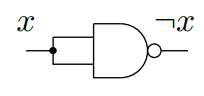
\includegraphics[width=0.6\linewidth, center]{./figures/not.png}
        \caption{NOT}
      \end{subfigure}
      \begin{subfigure}{0.3\linewidth}
        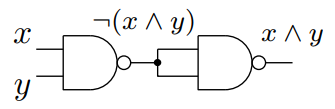
\includegraphics[width=0.9\linewidth, center]{./figures/and.png}
        \caption{AND}
      \end{subfigure}
      \begin{subfigure}{0.3\linewidth}
        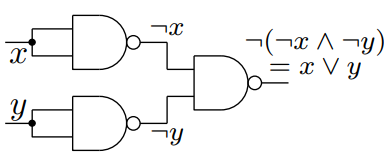
\includegraphics[width=\linewidth, center]{./figures/or.png}
        \caption{OR}
      \end{subfigure}
      \begin{subfigure}{0.3\linewidth}
        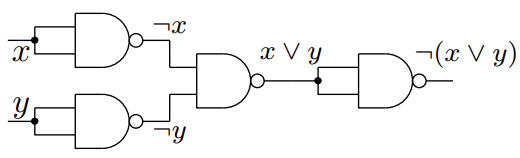
\includegraphics[width=\linewidth, center]{./figures/nor.png}
        \caption{NOR}
      \end{subfigure}
      \begin{subfigure}{0.3\linewidth}
        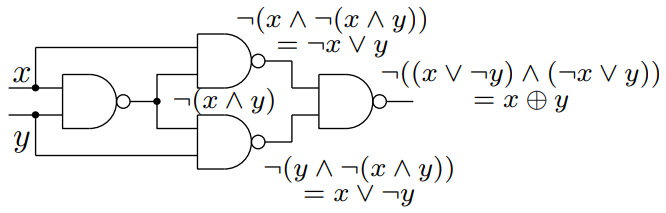
\includegraphics[width=\linewidth, center]{./figures/xor.png}
        \caption{XOR}
      \end{subfigure}
      \begin{subfigure}{0.3\linewidth}
        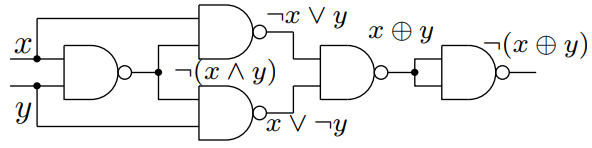
\includegraphics[width=\linewidth, center]{./figures/xnor.png}
        \caption{XNOR}
      \end{subfigure}
    \end{figure}
  \end{solutionnoinc}
  \begin{Sidenote}
    \begin{itemize}
      \item Aufgaben a) und b) zusammen zeigen, dass man mit Hilfe des $\operatorname{NAND}_2$ alle Funktionen $f: \mathbb{B}^2 \rightarrow \mathbb{B}$ realisieren kann.
    \end{itemize}
  \end{Sidenote}
\end{frame}
